% =============================================================================
% Lecture 09, Part 1: RNNs and LSTMs
% ECON 8310: Business Forecasting
% University of Nebraska at Omaha
% =============================================================================

\documentclass[aspectratio=169, 11pt]{beamer}

\input{header}

% ---- Lecture metadata --------------------------------------------------------
\title[RNNs \& LSTMs]{RNNs and LSTMs}
\subtitle{ECON 8310: Business Forecasting --- Lecture 9, Part 1}
\author{Department of Economics}
\institute{University of Nebraska at Omaha}

% =============================================================================
\begin{document}
% =============================================================================

\begin{frame}
  \titlepage
\end{frame}

% ---- Outline ----------------------------------------------------------------
\begin{frame}{Lecture Outline}
  \tableofcontents
\end{frame}

% =============================================================================
\section{Where the Last Two Lectures Ran Out}
% =============================================================================

\sectionslide{Where the Last Two Lectures Ran Out}{%
  Two architectures, two different ways of failing to see time.}

% --- Slide: the gap ----------------------------------------------------------
\begin{frame}{Two Architectures That Cannot See Time}
  Lecture 7's feedforward network treats each row independently: everything it knows about
  \emph{when}, you encoded by hand as lag columns.

  \vspace{0.2cm}
  Lecture 8's 1D CNN sees local shape, but its \textbf{receptive field} stops at about seven
  weeks, and pooling threw away \emph{where} each pattern occurred --- a measured 500 RMSE.

  \begin{keybox}
    Both treat the input as a \textbf{fixed-size block}, processed all at once. Neither reads a
    sequence \emph{in order}, carrying something forward. That is the gap today closes.
  \end{keybox}
\end{frame}

% --- Slide: the recurrent idea -----------------------------------------------
\begin{frame}{The Recurrent Idea: Carry State Forward}
  A recurrent network reads the sequence one step at a time, keeping a \textbf{hidden state}
  $\mathbf{h}_t$: a running summary of everything so far. Each step updates the summary from the
  new input \emph{and} the old summary, with the same weights every step --- weight sharing
  again, along time instead of space.

  \vspace{0.2cm}
  \textbf{The promise:} no fixed window. In principle $\mathbf{h}_t$ carries the whole history.

  \vspace{0.2cm}
  \textbf{In principle.} Most of this lecture is about the gap between that promise and what a
  recurrent network delivers --- and the architecture built to close it.
\end{frame}

% =============================================================================
\section{The Vanilla RNN}
% =============================================================================

\sectionslide{The Vanilla RNN}{%
  One equation, applied over and over --- and the reason
  that is both the whole idea and the whole problem.}

% --- Slide: RNN mechanics ----------------------------------------------------
\begin{frame}{Vanilla RNN: One Equation, Repeated}
  \begin{definitionbox}{The recurrence}
    \[
      \mathbf{h}_t = \tanh\!\left(\mathbf{W}_h \mathbf{h}_{t-1} + \mathbf{W}_x \mathbf{x}_t + \mathbf{b}\right),
      \qquad
      \hat{y}_t = \mathbf{W}_y \mathbf{h}_t + \mathbf{b}_y
    \]
  \end{definitionbox}
  \vspace{-0.2cm}
  \begin{center}
    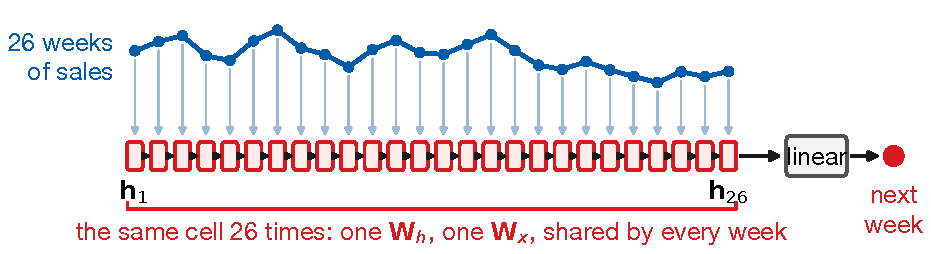
\includegraphics[height=3.2cm]{../Figures/Lecture09_Part1/unrolled_rnn.pdf}
  \end{center}
  \vspace{-0.2cm}
  In words: the new summary is a squashed mix of the old summary and the new week. Shared weights
  mean a 26-week window costs no more parameters than a 5-week one --- about \textbf{4{,}500}
  here, against 22{,}657 for Lecture 7's network.
\end{frame}

% --- Slide: BPTT -------------------------------------------------------------
\begin{frame}{Training It: Backpropagation Through Time}
  Training is ordinary backpropagation on an unusual graph. \textbf{Unroll} the recurrence and it
  is a 26-layer network, one layer per week, every layer sharing the same weights. Gradients flow
  back from step $T$ to step 1, and $\mathbf{W}_h$'s gradient sums contributions from all 26.

  \begin{warningbox}
    \textbf{This is where it breaks.} Going back $k$ steps multiplies by $\mathbf{W}_h$ and by
    $\tanh' \le 1$, $k$ times. Below 1, the gradient shrinks \emph{exponentially}; above 1, it can explode.
  \end{warningbox}

  Exploding is fixed by \texttt{clip\_grad\_norm\_}; vanishing is not --- the next section.
\end{frame}

% --- Slide: vanishing gradients ----------------------------------------------
\begin{frame}{Why a Vanilla RNN Forgets \parencite{Bengio1994}}
  Suppose each backward step multiplies the gradient by $0.7$ --- an unremarkable value for a
  $\tanh$ network --- and compare our own RNN, trained on 52-week windows, measured:
  \begin{center}
    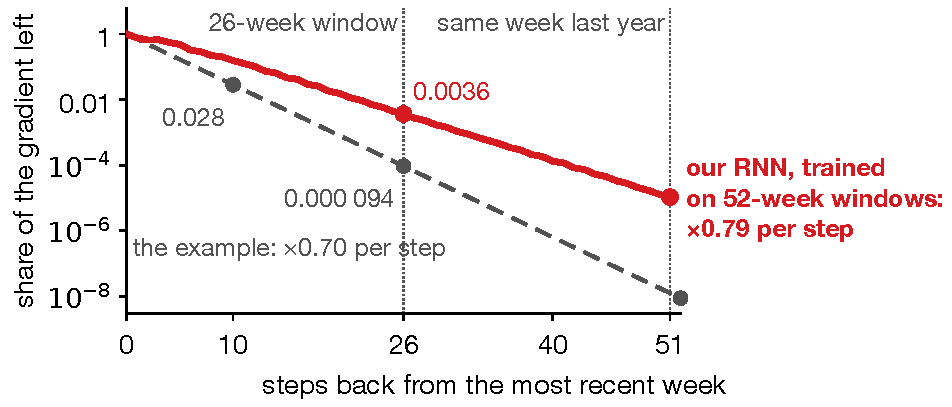
\includegraphics[height=4.3cm]{../Figures/Lecture09_Part1/gradient_decay.pdf}
  \end{center}
  \vspace{-0.25cm}
  \textbf{The same factor every step is a straight line on a log scale.} Past the first few steps,
  ours keeps about $0.79$ a step; measured, \textbf{0.4\%} of the gradient reaches 26 weeks back,
  \textbf{0.001\%} the same week last year. \textbf{Bengio and colleagues} proved this is inherent
  to the architecture.
\end{frame}

% =============================================================================
\section{LSTM: Long Short-Term Memory}
% =============================================================================

\sectionslide{LSTM: Long Short-Term Memory}{%
  Add a memory that information passes through rather than
  being recomputed at every step.}

% --- Slide: LSTM gates -------------------------------------------------------
\begin{frame}{LSTM: A Cell State and Three Gates}
  An LSTM carries \textbf{two} things forward: a \textbf{cell state} $\mathbf{c}_t$, which is the
  long-term memory, and a \textbf{hidden state} $\mathbf{h}_t$, which is what the rest of the
  network sees. Three gates control the traffic between them
  \parencite{Hochreiter1997,Gers2000}.
  \begin{center}
    {\small
    \begin{tabular}{p{2.3cm}p{10.2cm}}
      \toprule
      \textbf{Forget gate} & $\mathbf{f}_t = \sigma(\mathbf{W}_f[\mathbf{h}_{t-1}, \mathbf{x}_t] + \mathbf{b}_f)$
        --- what fraction of the old memory to keep \\[3pt]
      \textbf{Input gate} & $\mathbf{i}_t = \sigma(\mathbf{W}_i[\mathbf{h}_{t-1}, \mathbf{x}_t] + \mathbf{b}_i)$
        --- how much of the new candidate to write \\[3pt]
      \textbf{Output gate} & $\mathbf{o}_t = \sigma(\mathbf{W}_o[\mathbf{h}_{t-1}, \mathbf{x}_t] + \mathbf{b}_o)$
        --- how much of memory to expose \\[3pt]
      \textbf{Candidate} & $\tilde{\mathbf{c}}_t = \tanh(\mathbf{W}_c[\mathbf{h}_{t-1}, \mathbf{x}_t] + \mathbf{b}_c)$
        --- the new content on offer \\
      \bottomrule
    \end{tabular}
    }
  \end{center}

  \vspace{-0.1cm}
  The memory update itself is the line that matters:
  \[
    \mathbf{c}_t = \mathbf{f}_t \odot \mathbf{c}_{t-1} \;+\; \mathbf{i}_t \odot \tilde{\mathbf{c}}_t,
    \qquad
    \mathbf{h}_t = \mathbf{o}_t \odot \tanh(\mathbf{c}_t)
  \]
  \vspace{-0.3cm}

  Here $\sigma$ is the sigmoid, so each gate outputs between 0 and 1 --- a soft switch the network
  learns. $[\mathbf{h}_{t-1}, \mathbf{x}_t]$ stacks the two vectors; $\odot$ multiplies element by
  element.
\end{frame}

% --- Slide: gates in business terms -------------------------------------------
\begin{frame}{What the Gates Are Doing, in Plain Terms}
  The equations are compact but the behavior is intuitive. Take a store forecasting demand week
  by week.

  \vspace{0.1cm}
  \begin{center}
    {\small
    \begin{tabular}{p{2.4cm}p{10.1cm}}
      \toprule
      \textbf{Forget} & ``The promotion that ran three months ago no longer explains anything ---
      drop it.'' The gate closes toward 0 and that part of memory decays away. \\[3pt]
      \textbf{Input} & ``This week is Thanksgiving and the spike is enormous --- record it.'' The
      gate opens toward 1 and the event is written into the cell. \\[3pt]
      \textbf{Output} & ``I am holding a memory of last December, but this week is April --- do
      not act on it yet.'' Information stays in $\mathbf{c}_t$ without contaminating the current
      prediction. \\
      \bottomrule
    \end{tabular}
    }
  \end{center}

  \vspace{0.1cm}
  \textbf{The output gate is the one people skip, and it is the subtle one.} It separates
  \emph{what the model remembers} from \emph{what the model uses right now}. A vanilla RNN cannot
  make that distinction --- its single hidden state has to serve both jobs at once, so anything
  it stores is immediately in play.
\end{frame}

% --- Slide: why it fixes the gradient -----------------------------------------
\begin{frame}{Why the Cell State Fixes the Gradient}
  Follow a gradient backward through
  $\mathbf{c}_t = \mathbf{f}_t \odot \mathbf{c}_{t-1} + \mathbf{i}_t \odot \tilde{\mathbf{c}}_t$.
  Repeated multiplication shrinks; repeated addition does not.
  \begin{center}
    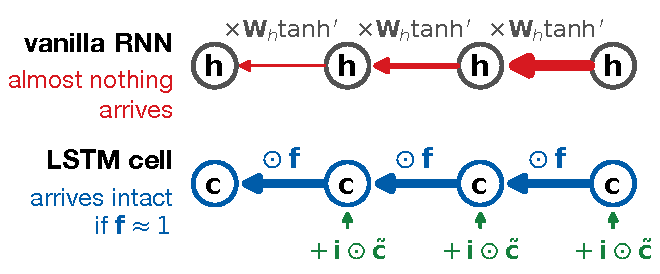
\includegraphics[height=3.5cm]{../Figures/Lecture09_Part1/cell_lanes.pdf}
  \end{center}
  \vspace{-0.3cm}
  \begin{keybox}
    \small\textbf{You have seen this fix before:} Lecture 8's skip connection,
    $\mathbf{y} = \mathcal{F}(\mathbf{x}) + \mathbf{x}$. The 1997 LSTM had no forget gate, so its
    cell path \emph{was} that identity, eighteen years before ResNet; the forget gate (2000) made
    it learnable.
  \end{keybox}
  \vspace{-0.1cm}
  {\small\muted{On our panel the median forget gate is 0.52, so 7\% survives four weeks. Check 2
  says why.}}
\end{frame}

% =============================================================================
\section{In PyTorch, and Does It Work}
% =============================================================================

\sectionslide{In PyTorch, and Does It Work}{%
  Four lines of model code, and an honest measurement against
  everything else this course has fitted.}

% --- Slide: PyTorch ----------------------------------------------------------
\begin{frame}{LSTM for Forecasting in PyTorch}
  \begin{examplebox}{Window in, one forecast out}
    {\tiny\linespread{1.2}\selectfont
    \texttt{class LSTMForecaster(nn.Module):}\\
    \texttt{\mbox{}\ \ def \_\_init\_\_(self, n\_features, hidden=64, layers=1):}\\
    \texttt{\mbox{}\ \ \ \ super().\_\_init\_\_()}\\
    \texttt{\mbox{}\ \ \ \ self.lstm = nn.LSTM(n\_features, hidden, num\_layers=layers,}\\
    \texttt{\mbox{}\ \ \ \ \ \ \ \ \ \ \ \ \ \ \ \ \ \ \ \ \ \ \ \ batch\_first=True)}\\
    \texttt{\mbox{}\ \ \ \ self.fc = nn.Linear(hidden, 1)}\\[3pt]
    \texttt{\mbox{}\ \ def forward(self, x):\ \ \ \ \ \ \# x: (batch, seq\_len, n\_features)}\\
    \texttt{\mbox{}\ \ \ \ out, (h, c) = self.lstm(x)\ \ \# nn.RNN instead: out, h = self.rnn(x)}\\
    \texttt{\mbox{}\ \ \ \ return self.fc(out[:, -1, :]).squeeze(-1)}
    }
  \end{examplebox}
  \texttt{batch\_first=True} gives shape \texttt{(batch, seq\_len, features)} --- the
  \emph{opposite} of \texttt{Conv1d}. \texttt{out[:, -1, :]} is the state after the last step.
  Lecture 7's rules still hold, plus \texttt{clip\_grad\_norm\_(..., 1.0)}.
\end{frame}

% --- Slide: results ----------------------------------------------------------
\begin{frame}{Does It Work? The Scoreboard So Far}
  Same weekly panel, same 26-week windows, same test block as Homework 4.
  \begin{center}
    {\small
    \begin{tabular}{lrr}
      \toprule
      \textbf{Model} & \textbf{Test RMSE} & \textbf{Parameters} \\
      \midrule
      LASSO, 46 engineered features & \textbf{744} & 46 \\
      XGBoost, 46 engineered features & 781 & --- \\
      \textbf{Vanilla RNN}, 4 raw channels & \textbf{842} & 4{,}545 \\
      Random forest & 899 & --- \\
      \textbf{LSTM}, 4 raw channels & 987 & 17{,}985 \\
      1D CNN, best variant & 1{,}032 & 8{,}161 \\
      Seasonal naive & 2{,}152 & 0 \\
      \bottomrule
    \end{tabular}
    }
  \end{center}

  \vspace{-0.05cm}
  \textbf{Recurrence beats convolution decisively} --- and it did so on \emph{four raw channels}
  with no lag engineering at all, against 46 hand-built features for LASSO. That is the case for
  reading a sequence in order, in one line.

  \vspace{0.1cm}
  \textbf{And the LSTM lost to the vanilla RNN} --- at a fixed 30-epoch budget. That is not a
  typo, and the next four slides are about what it does and does not mean.
\end{frame}

% --- Slide: why LSTM lost ----------------------------------------------------
\begin{frame}{Why the Gated Model Lost at 30 Epochs}
  All three windows share one panel and one split: one finding measured three ways, not three
  tests.
  \begin{center}
    {\small
    \begin{tabular}{lrrl}
      \toprule
      \textbf{Window} & \textbf{Vanilla RNN} & \textbf{LSTM} & \\
      \midrule
      13 weeks & \textbf{878} & 990 & RNN wins \\
      26 weeks & \textbf{842} & 987 & RNN wins \\
      52 weeks & \textbf{805} & 998 & RNN wins \\
      \bottomrule
    \end{tabular}
    }
  \end{center}

  \vspace{-0.3cm}
  \textbf{An LSTM solves a problem this data does not have}: gating preserves information across
  \emph{long} chains, and weekly demand is dominated by the recent past. The gates cost
  \textbf{17{,}985 parameters against 4{,}545}. Two checks first: \textbf{was the comparison
  fair}, and \textbf{what in the data explains it}?

  \begin{warningbox}
    A margin measured at one training budget is a claim about that budget --- and 30 epochs was
    just the default.
  \end{warningbox}
\end{frame}

% --- Slide: the budget check -------------------------------------------------
\begin{frame}{Check 1: Was It a Fair Fight?}
  Bigger models converge slower, and the LSTM has $4\times$ the parameters. Vary the
  \textbf{budget}:
  \begin{center}
    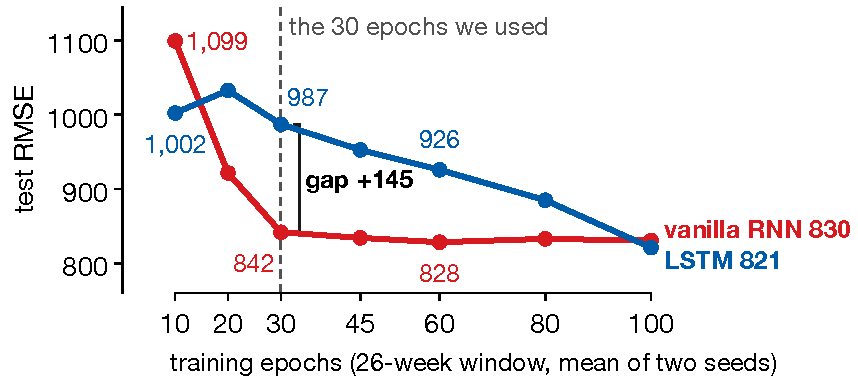
\includegraphics[height=4.0cm]{../Figures/Lecture09_Part1/budget_curve.pdf}
  \end{center}
  \vspace{-0.3cm}
  \begin{keybox}
    At 30 epochs the RNN wins by a wide margin. By 100 the two \textbf{tie}, and the LSTM is still
    improving: we ran out of patience, not the model. The RNN's real edge is speed ---
    \textbf{three times faster on a quarter of the parameters} --- not a verdict on gating.
  \end{keybox}
\end{frame}

% --- Slide: the data check ---------------------------------------------------
\begin{frame}{Check 2: What in the Data Explains It}
  Gating pays when a value must survive many steps that would otherwise overwrite it. Does this
  panel have that?
  \begin{center}
    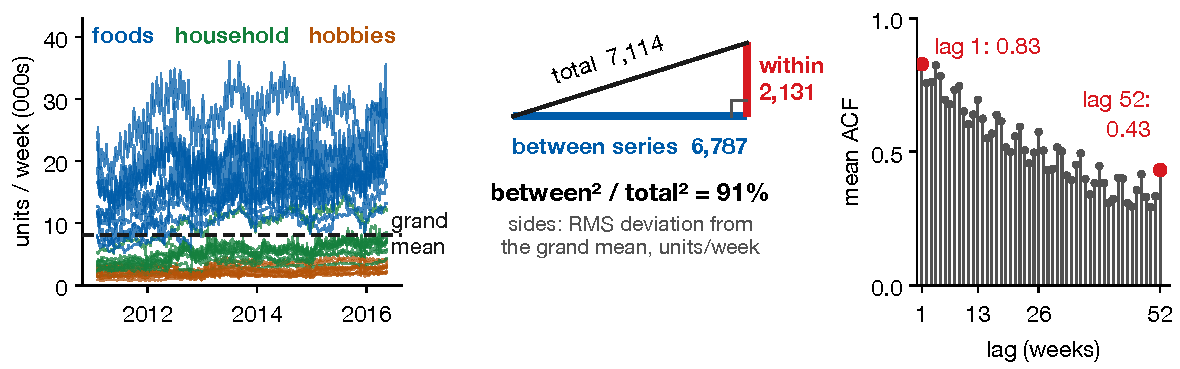
\includegraphics[height=4.0cm]{../Figures/Lecture09_Part1/panel_variance.pdf}
  \end{center}
  \vspace{-0.35cm}
  \textbf{1. Most variance is not sequential.} \textbf{91\%} is \emph{between} series: the task
  is reading the level, and the last few weeks give you that.

  \vspace{0.1cm}
  \textbf{2. History helps, but it arrives smoothly.} A longer window still improves the RNN
  (878 $\to$ 805), but no value has to survive many steps untouched.
\end{frame}

% --- Slide: the data check, continued -----------------------------------------
\begin{frame}{Check 2, Continued: Nothing Arrives Early}
  \textbf{3. Nothing arrives early.} \texttt{snap\_days} correlates $+0.14$ with units in the
  same week. Its $-0.13$ and $+0.12$ two and four weeks ahead only echo that through the monthly
  SNAP calendar, and \texttt{event\_days} is flat everywhere. No \emph{announcement} structure ---
  exactly what a forget gate is for.

  \begin{keybox}
    Ask these of your own series before reaching for a gated model: How much of my variance is
    cross-sectional? Do recent values already summarize old ones? Does anything in my inputs
    \textbf{lead} the target?
  \end{keybox}
\end{frame}

% =============================================================================
\section{Key Takeaways}
% =============================================================================

\sectionslide{Key Takeaways}{%
  What recurrence buys, what it costs, and what is still missing.}

% --- Slide: comparison -------------------------------------------------------
\begin{frame}{RNN and LSTM in Context}
  \begin{center}
    {\small
    \begin{tabular}{llll}
      \toprule
      \textbf{Architecture} & \textbf{Sees order?} & \textbf{Effective memory} & \textbf{Cost} \\
      \midrule
      FFN on lags & no & whatever you engineered & cheap \\
      1D CNN & local only & receptive field ($\sim$7 steps) & cheap \\
      Vanilla RNN & yes & $\sim$10--30 steps in practice & cheap \\
      LSTM & yes & hundreds of steps & 4$\times$ an RNN \\
      \bottomrule
    \end{tabular}
    }
  \end{center}

  \vspace{0.15cm}
  An LSTM holds about \textbf{four times} an RNN's parameters at the same hidden size: three gates
  and the candidate each need a weight matrix. On a short window you pay that for nothing.

  \vspace{0.15cm}
  \textbf{Still missing:} an LSTM reads strictly left to right, so it cannot be parallelized, and
  everything about step 3 must squeeze through every state between 3 and $T$. Part 2 removes
  both.
\end{frame}

% --- Slide: takeaways --------------------------------------------------------
\begin{frame}{Lecture 9, Part 1: Key Takeaways}
  \begin{keybox}
    {\small
    \begin{enumerate}\itemsep3pt
      \item A \textbf{recurrent network} reads in order, carrying a hidden state.
      \item \textbf{Backpropagation through time} multiplies at every step, so the gradient
            shrinks exponentially --- ours keeps 0.001\% of it a year back.
      \item An \textbf{LSTM}'s cell state is updated \textbf{additively}: the ResNet fix,
            eighteen years earlier.
      \item Three gates: \textbf{forget} the stale, \textbf{input} the new, \textbf{output} what
            matters now.
      \item Both \textbf{beat every CNN}; both lose to a 46-coefficient LASSO.
      \item The LSTM \textbf{lost at 30 epochs and tied by 100}. Check a margin survives the training
            budget.
    \end{enumerate}
    }
  \end{keybox}
\end{frame}

% --- References ---------------------------------------------------------------
\begin{frame}[allowframebreaks]{References}
  \printbibliography[heading=none]
\end{frame}

\end{document}
